% An introduction to rhiza-claude — the narrative companion to the reference docs.
%
% Addresses issue #74: both entry points list *what* the plugin contains without
% explaining *what it is for*. This is the long form of the introduction that now
% opens docs/index.md; the README carries the short form.
%
% Build (either works, no shell-escape, no external data):
%   pdflatex rhiza-claude-intro.tex   # twice, for the ToC and page refs
%   tectonic rhiza-claude-intro.tex
%
% Every claim here is true of release v0.6.1. When the plugin changes, this file is
% part of the change — a stale introduction is worse than none.

\documentclass[11pt,a4paper]{article}

\usepackage[T1]{fontenc}
\usepackage[utf8]{inputenc}
\usepackage{lmodern}
\usepackage[margin=2.4cm]{geometry}
\usepackage{booktabs}
\usepackage{enumitem}
\usepackage{xcolor}
\usepackage{listings}
\usepackage{tikz}
\usepackage{fancyhdr}
\usepackage[hidelinks]{hyperref}

\usetikzlibrary{positioning, arrows.meta, fit, backgrounds}

\definecolor{leaf}{RGB}{31,105,68}
\definecolor{slate}{RGB}{70,78,86}
\definecolor{shell}{RGB}{245,245,242}

\lstdefinestyle{shellstyle}{
  basicstyle=\ttfamily\small,
  backgroundcolor=\color{shell},
  frame=single,
  rulecolor=\color{slate!25},
  framesep=5pt,
  xleftmargin=6pt,
  breaklines=true,
  columns=fullflexible,
  keepspaces=true,
  literate={→}{{$\to$}}1 {—}{{---}}1 {…}{{\ldots}}1,
}
\lstset{style=shellstyle}

\newcommand{\cmd}[1]{\texttt{/rhiza:#1}}
\newcommand{\file}[1]{\texttt{#1}}

\pagestyle{fancy}
\fancyhf{}
\fancyhead[L]{\small\color{slate}An introduction to rhiza-claude}
\fancyhead[R]{\small\color{slate}v0.6.1}
\fancyfoot[C]{\small\color{slate}\thepage}
\renewcommand{\headrulewidth}{0.3pt}
\renewcommand{\headrule}{\hbox to\headwidth{\color{slate!30}\leaders\hrule height \headrulewidth\hfill}}

\title{\vspace{-1.4cm}\textbf{An introduction to rhiza-claude}\\[0.3em]
\large\color{slate} What the plugin is for, before what it contains}
\author{\normalsize Jebel Quant}
\date{\normalsize Release v0.6.1}

\begin{document}
\maketitle
\thispagestyle{fancy}

\begin{abstract}
\noindent
\textbf{rhiza-claude} is a Claude Code plugin for repositories that share their
scaffolding with a template repository instead of each carrying a private copy of it.
This document is the part the reference pages cannot be: not a catalogue of the seven
markdown files under \file{commands/}, but an account of the problem they exist to
solve --- the two-repository boundary a sync respects, what ``rhiza-managed'' actually
means on disk, the order the commands are meant to be run in, and why a plugin whose
selling point is determinism keeps half of itself in prose. It closes with a worked
first run: empty directory to a managed, synced, scored repository.
\end{abstract}

\section{The problem}

Ten repositories need substantially the same scaffolding. Continuous integration
workflows, a \file{Makefile}, lint and type and coverage gates, a documentation build,
a licence, a release path. None of it is the interesting part of any of those ten
projects, and all of it has to exist before the interesting part can be trusted.

The obvious approach --- write it once, copy it into each repository --- fails slowly
rather than loudly. A workflow gets fixed in one repository and not the other nine. A
coverage threshold gets lowered under deadline in a repository nobody revisits. Two
years later there is no answer to the question \emph{which repositories have the
current gates}, because nothing anywhere records which vintage of the scaffolding each
one received.

\textbf{rhiza} is that scaffolding kept once, in a \emph{template repository}:
\href{https://github.com/jebel-quant/rhiza}{\texttt{jebel-quant/rhiza}} for Python,
\texttt{rhiza-go} for Go. \textbf{rhiza-claude} --- this plugin --- is how an
individual repository adopts that template, keeps up with its releases, and is told how
well it is doing against the gates the template delivers.

Two things follow from that framing, and they are the reason an introduction is needed
at all. First, there are always \emph{two} repositories in play, and almost every
question a newcomer has is really a question about the boundary between them. Second,
the interesting work is not the copying --- it is knowing precisely which files are the
template's to overwrite and which are yours to keep.

\section{The two-repository model}

\begin{center}
\begin{tabular}{@{}p{0.30\linewidth}p{0.36\linewidth}p{0.26\linewidth}@{}}
\toprule
& \textbf{owns} & \textbf{who changes it} \\
\midrule
\textbf{the template} &
CI stubs, \file{Makefile}, \file{.rhiza/rhiza.mk}, the docs base &
upstream --- you receive it \\[0.4em]
\textbf{your repository} &
source, tests, \file{pyproject.toml}, README prose &
you --- the sync never touches it \\
\bottomrule
\end{tabular}
\end{center}

\noindent
A sync is therefore \emph{not} a copy of the template over your repository. \cmd{update}
writes only template-owned paths, and it knows which paths those are because the
previous sync wrote them down. Your \file{src/} is not in that set, so it cannot be
swept in --- there is no blanket \texttt{git add -{}-all} anywhere in the flow, which is a
deliberate design constraint rather than an implementation detail.

\begin{center}
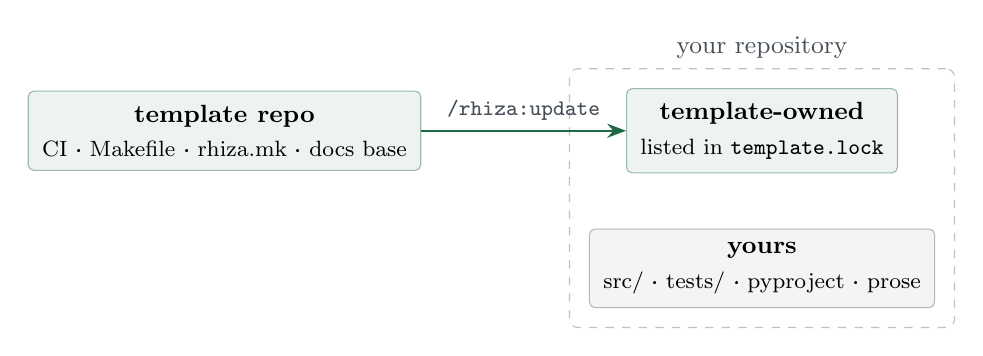
\begin{tikzpicture}[
  node distance=8mm,
  box/.style={draw=slate!40, rounded corners=2pt, align=center, inner sep=5pt,
              font=\small, minimum height=8mm},
  owned/.style={box, fill=leaf!8, draw=leaf!45},
  yours/.style={box, fill=slate!6},
  arrow/.style={-{Stealth[length=2.4mm]}, draw=leaf, thick},
]
\node[owned] (tpl) {\textbf{template repo}\\[0.15em]\footnotesize CI \textperiodcentered\ Makefile \textperiodcentered\ rhiza.mk \textperiodcentered\ docs base};
\node[owned, right=26mm of tpl] (managed) {\textbf{template-owned}\\[0.15em]\footnotesize listed in \file{template.lock}};
\node[yours, below=7mm of managed] (mine) {\textbf{yours}\\[0.15em]\footnotesize src/ \textperiodcentered\ tests/ \textperiodcentered\ pyproject \textperiodcentered\ prose};
\begin{scope}[on background layer]
  \node[draw=slate!35, dashed, rounded corners=3pt, fit=(managed)(mine),
        inner sep=7pt, label={[font=\small\color{slate}]above:your repository}] {};
\end{scope}
\draw[arrow] (tpl) -- node[above, font=\footnotesize, color=slate] {\cmd{update}} (managed);
\end{tikzpicture}
\end{center}

\noindent
The dashed boundary is your repository; the arrow is the only thing a sync does. Nothing
crosses into the lower box.

\section{What ``rhiza-managed'' means}

It means two files under \file{.rhiza/}, and they answer different questions.

\begin{center}
\begin{tabular}{@{}p{0.24\linewidth}p{0.34\linewidth}p{0.34\linewidth}@{}}
\toprule
\textbf{file} & \textbf{it is} & \textbf{question it answers} \\
\midrule
\file{template.yml} & a \textbf{pointer}: template repository and pinned \texttt{ref} & what \emph{would} we sync from? \\[0.4em]
\file{template.lock} & a \textbf{record}: repository, ref, commit SHA, timestamp, strategy, every managed file & what \emph{was} delivered, and when? \\
\bottomrule
\end{tabular}
\end{center}

\noindent
\textbf{Intent versus outcome.} The two disagree in both directions, which is the whole
reason both exist. A freshly initialised repository has a valid pointer and no lock at
all. A long-synced repository can carry a lock beside a pointer somebody has since
broken by hand. Reporting either one alone is misleading, so \cmd{status} always reports
both halves.

The same distinction is load-bearing for \cmd{quality}, which refuses to run unless it
finds \emph{both} \file{.rhiza/template.yml} and \file{.rhiza/rhiza.mk}. Every gate it
scores is a \texttt{make} target that the sync delivers; scoring a managed-but-unsynced
repository would report it as \emph{broken} when it is merely \emph{unsynced}, and that
is a wrong answer rather than a missing one. By contrast \cmd{release} requires neither
file: it reads the repository's own \texttt{[tool.bumpversion]} configuration, so it
works on any git repository, including this plugin.

\section{The intended path}

\begin{center}
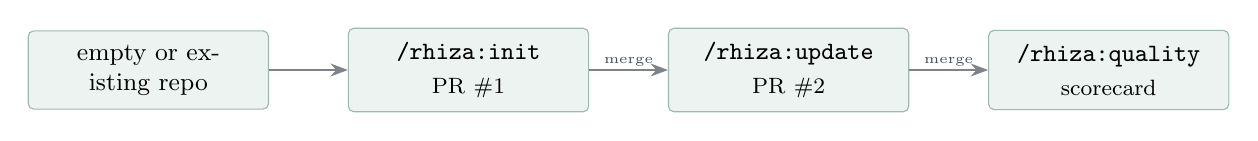
\begin{tikzpicture}[
  node distance=6mm,
  stepbox/.style={draw=leaf!45, fill=leaf!8, rounded corners=2pt, align=center,
               font=\small, inner sep=5pt, text width=27mm},
  gate/.style={align=center, font=\tiny\color{slate}, inner sep=1pt},
  arrow/.style={-{Stealth[length=2.2mm]}, draw=slate!70},
]
\node[stepbox] (a) {empty or existing repo};
\node[stepbox, right=10mm of a] (b) {\cmd{init}\\[0.15em]\footnotesize PR \#1};
\node[stepbox, right=10mm of b] (c) {\cmd{update}\\[0.15em]\footnotesize PR \#2};
\node[stepbox, right=10mm of c] (d) {\cmd{quality}\\[0.15em]\footnotesize scorecard};
\draw[arrow] (a) -- (b);
\draw[arrow] (b) -- node[gate, above] {merge} (c);
\draw[arrow] (c) -- node[gate, above] {merge} (d);
\end{tikzpicture}
\end{center}

Three commands, two pull requests you merge yourself, in that order:

\begin{enumerate}[leftmargin=1.4em, itemsep=0.35em]
  \item \cmd{init} writes exactly one file of its own --- \file{.rhiza/template.yml} ---
        and \textbf{deliberately syncs nothing}. No CI, no \file{Makefile}, no gates
        arrive at this step.
  \item \cmd{update} performs the first sync. This is what brings the template content
        in and what writes \file{.rhiza/template.lock}.
  \item \cmd{quality} needs that content to exist as real \texttt{make} targets, so it
        comes third.
\end{enumerate}

\noindent
Running them out of order is not dangerous --- each stops early and says why --- but the
sequence is worth knowing in advance, because \emph{``\cmd{init} ran and no CI
appeared''} is the expected outcome of step one rather than a failure. Separating the two
pull requests is the point: the file that declares which template you follow is
reviewable on its own, apart from the several dozen files that template then delivers.

\section{A worked first run}

\subsection*{0. A git repository with a remote}

\begin{lstlisting}
mkdir my-lib && cd my-lib && git init
gh repo create my-lib --private --source=. --push   # or create it in the UI
\end{lstlisting}

\noindent
\cmd{init} never pushes to your default branch. If the repository does not exist
upstream yet it asks \emph{you} to create it --- an empty README is enough --- rather
than pushing one itself. Then start Claude Code in that directory.

\subsection*{1. \cmd{init} --- become rhiza-managed}

It detects platform, owner and name from \texttt{origin} (asking when it cannot), picks
the language and template repository, resolves the template's latest release as the
initial pin, and opens a pull request on a \texttt{rhiza\_init\_<date>} branch:

\begin{center}
\begin{tabular}{@{}p{0.32\linewidth}p{0.60\linewidth}@{}}
\toprule
\textbf{written by} & \textbf{file} \\
\midrule
the command itself & \file{.rhiza/template.yml} --- the pointer and pinned ref \\
the skeleton procedure & \file{pyproject.toml} (via \texttt{uv init -{}-lib}), \file{src/}, \file{.python-version} \\
the license procedure & \file{LICENSE} plus the SPDX metadata in \file{pyproject.toml} \\
\bottomrule
\end{tabular}
\end{center}

\noindent
There is no \file{.rhiza/template.lock} yet, and no workflows. Merge the pull request.

\subsection*{2. \cmd{update} --- the first sync}

It bumps the \texttt{ref} in \file{template.yml} to the newest template release, syncs,
resolves any conflict by taking the upstream side, and opens a second pull request
carrying the template-owned files --- \file{.github/workflows/}, \file{Makefile},
\file{.rhiza/rhiza.mk}, the docs base --- together with \file{.rhiza/template.lock}
recording exactly what was delivered. Only paths the lock names are staged, so nothing
of yours is included even if it changed in your working tree. Merge that too.

\subsection*{3. \cmd{status} --- confirm both halves}

\begin{lstlisting}
/rhiza:status --files
\end{lstlisting}

\noindent
Read-only. It validates the pointer \emph{and} prints what the lock records: repository,
ref, commit SHA, timestamp, strategy, and with \texttt{-{}-files} the managed files as a
tree. This is how you distinguish \emph{managed and synced} from \emph{managed but never
synced}.

\subsection*{4. \cmd{quality} --- get scored}

Now that the gates exist, this runs them --- lint, types, documentation, dependencies,
security, tests, test layout, complexity, architecture --- and produces a 1--10
scorecard with findings and an optional menu to file them as issues. It proposes fixes
and applies none.

\medskip
\noindent
Afterwards: \cmd{update} again whenever the template cuts a release
(\texttt{-{}-check} compares your pin against the latest), \cmd{docs} to
create or refresh \file{README.md}, \file{CLAUDE.md} and \file{mkdocs.yml}
(preserving hand-written prose), and \cmd{release} when you want to cut a version.

\section{Commands and procedures}

The plugin ships two kinds of markdown, and the distinction is enforced rather than
conventional:

\begin{itemize}[leftmargin=1.4em, itemsep=0.3em]
  \item \file{commands/*.md} are \textbf{slash commands} you invoke: seven of them, each
        with a reference page.
  \item \file{prompts/*.md} are \textbf{internal procedures}: seven shared steps a
        command reaches with the \texttt{Read} tool, kept deliberately \emph{outside}
        \file{commands/} so they cannot be invoked directly.
\end{itemize}

\noindent
Procedures are not implementation trivia, and filing them under ``internals'' undersells
them: they are where the shared behaviour lives, which is why \file{init.md} alone does
not explain what \cmd{init} does. Installing \texttt{uv}, choosing a work branch off an
untouched default, scaffolding a \file{pyproject.toml}, writing a licence, gathering
design evidence, applying the scoring rubric --- each is a procedure, and that is
exactly why \cmd{init} and \cmd{update} behave identically everywhere they overlap. A
check in CI enforces the arrangement: no procedure may carry command frontmatter, none
may collide with a command name, every referenced procedure path must resolve, and no
procedure may be orphaned.

\section{The seven commands, and what each writes}

An introduction should say which of these change your repository, because that is the
first thing anyone actually wants to know.

\begin{center}
\small
\begin{tabular}{@{}p{0.20\linewidth}p{0.40\linewidth}p{0.32\linewidth}@{}}
\toprule
\textbf{command} & \textbf{what it does} & \textbf{what it writes} \\
\midrule
\cmd{init} & make the repository rhiza-managed; no sync, no gates &
one file of its own, then a pull request \\[0.35em]
\cmd{update} & sync to a template release, upstream side wins conflicts &
template-owned paths only, then a pull request \\[0.35em]
\cmd{quality} & run the gates and score 1--10 with findings &
nothing --- proposes fixes, applies none \\[0.35em]
\cmd{docs} & create or refresh \file{README.md}, \file{CLAUDE.md}, \file{mkdocs.yml} &
those files; no commit, no pull request \\[0.35em]
\cmd{release} & pick a next version from a table, bump, changelog &
one local commit and one tag; never pushes \\[0.35em]
\cmd{status} & report the pointer \emph{and} the lock &
nothing --- read-only \\[0.35em]
\cmd{uninstall} & delete every file the lock records, prune empty dirs &
removes files; confirms first \\
\bottomrule
\end{tabular}
\end{center}

\noindent
Two patterns are worth reading off that table. The commands that change a \emph{shared}
repository do it through a pull request you review --- neither \cmd{init} nor
\cmd{update} pushes to your default branch. And the ones that assess rather than act
(\cmd{quality}, \cmd{status}) write nothing at all, which is what makes them safe to run
on a repository you have just inherited and do not yet understand.

\subsection*{Common confusions}

\begin{description}[leftmargin=0pt, style=nextline, itemsep=0.35em]
  \item[``\cmd{init} finished but no CI appeared.'']
        Correct behaviour. \cmd{init} writes the pointer; \cmd{update} performs the
        first sync. The template content arrives in the second pull request.
  \item[``Which CLI do I have to install?'']
        None. \texttt{uv} is the only hard dependency; the plugin's own scripts are
        stdlib-only Python. There is no \texttt{rhiza} CLI in this picture.
  \item[``Can I edit a synced file?'']
        You can, but \cmd{update} resolves conflicts by taking the upstream side, so
        your edit is expected to lose. Template-owned files are changed
        \emph{upstream}; that is the point of having one original.
  \item[``Will a sync overwrite my README?'']
        No. \file{README.md} is yours, not template-owned. \cmd{docs} is the only
        command that writes it, and it preserves hand-written prose --- it replaces the
        generated badge block and corrects stale facts, but never deletes what a human
        wrote.
  \item[``\cmd{quality} refuses to run.'']
        It found the pointer but no \file{.rhiza/rhiza.mk} --- managed, never synced.
        Run \cmd{update} first. The refusal is deliberate --- scoring at that
        point would report every missing gate as a failure of your code.
\end{description}

\section{Why the commands are prose}

The split is deliberate: \textbf{deterministic work belongs in tested code, judgement
belongs in markdown.}

The bundled Python under \file{scripts/} does the parts with exactly one right answer
--- parsing the lock, merging synced files, comparing versions as semver, computing the
legal candidate bumps --- and it is stdlib-only, strictly type-checked, and held at
100\,\% test coverage. The markdown does the parts that require a reading of your
repository: which findings matter, whether a breaking change should spend the 1.0
signal, what to preserve in a README a human wrote.

Two consequences are worth stating, because they are what make the arrangement more than
a slogan. First, \emph{the prose is gated too}: a command that names a script, a flag or
another command which no longer exists fails the build rather than failing in front of a
user mid-task. Second, where a model would reliably guess badly, the guess is removed
rather than improved --- \cmd{release} lays the legal next versions out as a table and
declines to recommend one, because whether \texttt{0.x} should become \texttt{1.0.0} is
an intention about API stability that no commit log records.

\section{What it needs, and what it is not}

\textbf{\texttt{uv} is the one hard dependency}, and both \cmd{init} and \cmd{update}
offer to install it as their first step. \texttt{git} and \texttt{make} are used and are
near-universal. The plugin's own scripts are stdlib-only Python: \textbf{there is no
\texttt{rhiza} CLI to install}, which is the most common point of confusion about what
this actually requires.

Honest scope, at v0.6.1: seven user-facing commands, seven internal procedures. It is
not a build system, a package manager, or a replacement for your CI --- the template
delivers workflows, and the plugin's job is to get them to you intact and tell you how
the result scores. Nothing here runs on a schedule or in the background; every command
is something you invoke, and the two commands that change a shared repository
(\cmd{init}, \cmd{update}) do it by opening a pull request you review.

\section{Glossary}

The words that carry the model, in one place. Each is used above in exactly this sense.

\begin{description}[leftmargin=0pt, style=nextline, itemsep=0.3em]
  \item[template repository]
        The upstream repository holding the shared scaffolding ---
        \texttt{jebel-quant/rhiza} for Python, \texttt{rhiza-go} for Go, or a fork of
        either. You read from it; you do not sync \emph{to} it.
  \item[pointer --- \file{template.yml}]
        Declared intent: which template repository, and which pinned \texttt{ref}. The
        one file \cmd{init} writes itself, and the file \cmd{update} bumps.
  \item[lock --- \file{template.lock}]
        Recorded outcome: repository, ref, commit SHA, timestamp, strategy, and the list
        of managed files. Written by a sync, never by hand.
  \item[managed file]
        A path the lock names --- template-owned, and therefore the sync's to overwrite.
        Everything not in that list is yours, and no command stages it.
  \item[rhiza-managed vs.\ synced]
        \emph{Managed} means the pointer exists. \emph{Synced} means the content
        arrived, which is observable as \file{.rhiza/rhiza.mk}. Both are required by
        \cmd{quality}, and the gap between the two is the state \cmd{init}
        deliberately leaves you in.
  \item[procedure --- \file{prompts/}]
        A shared step a command reaches with the \texttt{Read} tool, kept outside
        \file{commands/} so it cannot be invoked as a slash command.
  \item[gate]
        A \texttt{make} target delivered by the sync that either passes or fails: lint,
        types, docstring coverage, tests, dependency and security checks, test layout.
  \item[scorecard]
        What \cmd{quality} produces: a 1--10 mark per category with findings, plus an
        optional menu to file them as issues. Assessment only --- it applies no fixes.
\end{description}

\bigskip
\noindent
\small\color{slate}
Reference documentation for every command:
\href{https://jebel-quant.github.io/rhiza-claude/}{jebel-quant.github.io/rhiza-claude}.
The short form of this introduction opens the repository's \file{README.md}; the full
form opens \file{docs/index.md}.

\end{document}
